\section{Results}

\subsection{Modeling}

\begin{figure}[h!] 
	\centering
	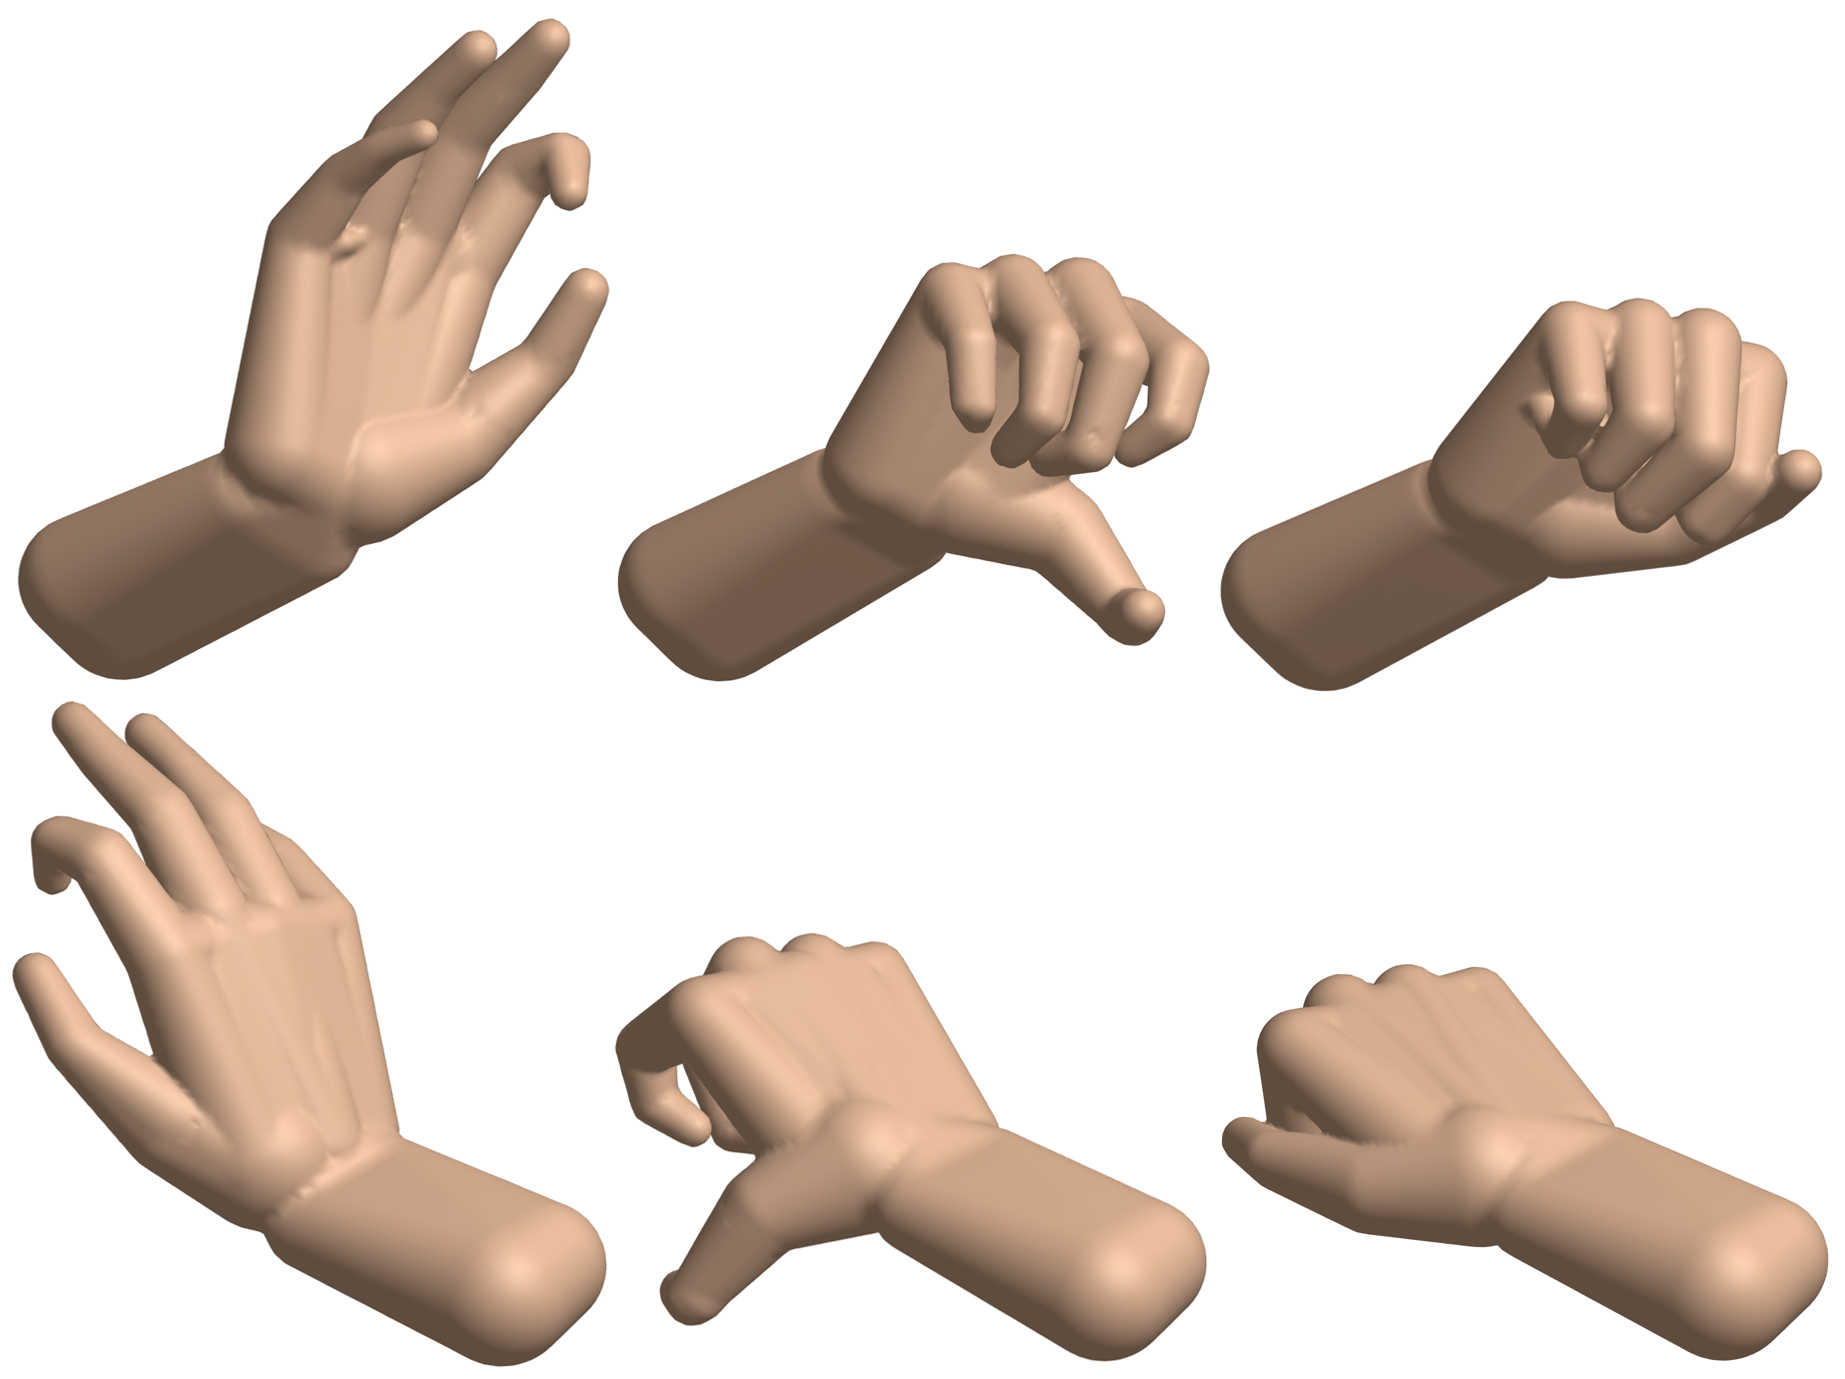
\includegraphics[width=0.5\textwidth]{figures/modeling}
	\caption{Fitting convolution surfaces hand model to several poses of the same hand.}
	\label{fig:modeling}
\end{figure}

\subsection{Tracking}

In this paper instead of a standard inverse kinematics approach for aligning the model with data we use \textit{"As Rigid As Possible"} approach. The hand model is parametrized with the locations of the vertices of the hand skeleton $c = {c_1, c_2, ... c_N}$.

\begin{equation}
	\min_{c} E_{ICP} + E_{ARAP} \label{eq:tracking_energy}
\end{equation}

The first energy $E_{ICP}$ models a 3D geometric registration in the spirit of ICP as

\begin{equation}
	E_{ICP} = \omega_1 \sum_{p \in P} \| p - \Pi(p, c)\|_2
\end{equation}

where $P$ is the set of data points.

The second energy $E_{ARAP}$ is needed for shape preservation. Denote locations of hand skeleton vertices at rest pose as $c^0$ and in iteration $t$ as $c^t$. Denote the set of all edges of hand skeleton as $E$.

\begin{equation}
	E_{ARAP} = \omega_2 \sum_{e \in E} \| e(c^t) - R_e e(c^0)\|_2^2,
\end{equation}

where $R_e$ is the optimal rotation to bring the rest pose edge $e^0$ to the current position $e^t$. Unless we what some set of edges to rotate as a solid body, the rotation $R_e$ can be expressed in the closed form, such that $R_e e(c^0)$ is collinear to $e(c^t)$. 
Each optimization iteration consists of two alternating steps: first we find the projections of the data points to the model surface $\Pi(p, c)$ and the optimal rotations $  R_e  $. Then we make one step of Levenberg-Marquardt iteration for energy (\ref{eq:tracking_energy}).

\subsubsection{Trying to make several optimization steps while keeping the same correspondences}

I am not sure how to implement what you suggested yesterday. If the data-model correspondences are kept fixed, after the first update of the parameters the model points are not in the model surface anymore. So, the optimization does not make much sense (see Figure \ref{fig:fixed_correspondences}). If I do such optimization, the model just floats away from the data.
I also tried doing several iterations of $E_{ARAP}$ only, The initial length of the segment are, of course, restored. However, the model does not take the data into account during these iterations, so the optimization takes more time to converge.

\begin{figure}[h!] 
	\centering
	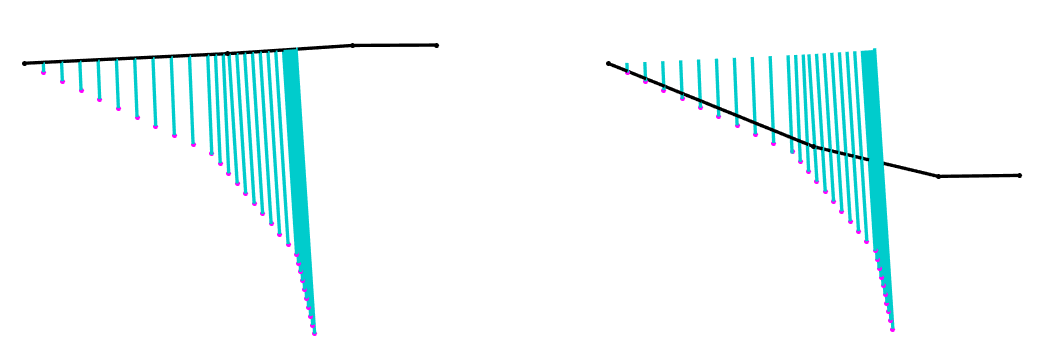
\includegraphics[width=0.5\textwidth]{figures/fixed_correspondences}
	\caption{Updating the centers locations while keeping the data-model correspondences fixed. The model is black, the data is pink, the corresponding points are connected in blue.}
	\label{fig:fixed_correspondences}
\end{figure}